\documentclass[a4paper]{article}
\usepackage[english]{babel}
\usepackage[utf8]{inputenc}
\usepackage{amsmath}
\usepackage{graphicx}
\usepackage{natbib}
\usepackage{float}
\usepackage[margin=1.2in]{geometry}
\usepackage{caption}
\usepackage{subcaption}
\usepackage{url}
\usepackage{bm}
\usepackage{wasysym}
\usepackage{pdflscape}
\usepackage{tabularx}
\usepackage{hhline}
\usepackage{geometry}
\usepackage{longtable}
\usepackage{amsmath,bm}
\usepackage{array}
\usepackage{mathtools}
\usepackage{setspace}
%\usepackage{hyperref}
\onehalfspacing

\mathchardef\mhyphen="2D

\newcommand{\pder}[2][]{\frac{\partial#1}{\partial#2}}
\newcommand{\pdder}[2][]{\frac{\partial^2#1}{\partial#2 ^2}}
\newcolumntype{P}[1]{>{\centering\arraybackslash}p{#1}}

\graphicspath{{./plots/}}

%----------------------------------------------------------------------------------------

\title{Time Series\\ Exercise 2}

\author{Rory Hetherington (200471193)}

\date{27 Feb 2017}

\begin{document}


\maketitle

%----------------------------------------------------------------------------------------

\section*{Question 1}

\begin{figure}
	\centering
	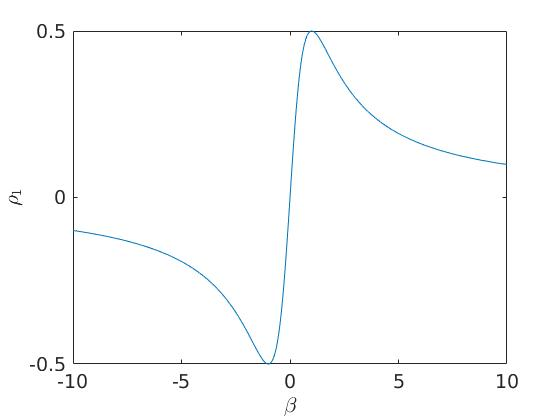
\includegraphics[width=0.6\textwidth]{ex_2_4}
	\caption{$\rho_1$ as a function of  $\beta$.}
	\label{fig:ex_2_4}
\end{figure}


\end{document}